\lecture{1}{29. August 2025}{Fourier Theory}

\exercise{1.}
Consider the following periodic functions. Find possible values for the period, using the definition of periodic functions.

\begin{enumerate}[label=(\alph*)]
  \item $f(x) = e^{\cos x}$
  \item $f(x) = \cos \left( x + \frac{\pi}{3} \right)$
  \item $f(x) = \cos \frac{\pi x}{3}$
  \item $f(x) = \cos x + \cos 3x$
  \item $f(x) = \cos x \cos 3x$
  \item $f(x) = \cos x + \cos \left( \num{0,6} x \right)$
\end{enumerate}

For (a) the exponent to $e$, i.e. $\cos x$ only has a range of $(-1; 1)$. This means that the exponent will change between $-1$ and $1$ with a period of $2\pi$, therefore the period $p_a = 2\pi$ will also be the case for the function described in (a).

For (b) we are once again working with a $\cos$ function. This time it is however shifted by $\frac{\pi}{3}$ along the $x$-axis. A translation along the $x$-axis will, however, not affect the period of the function and therefore the period here is once again $p_b = 2\pi$.

For (c) the $x$ is multiplied by $\frac{\pi}{3} \approx \num{1,047}$. This means that the argument to the cosine will reach $2\pi$ at a speed that is $\frac{\pi}{3} \approx \num{1,047}$ times faster than a normal cosine. Therefore the period of this is $p_c = \frac{3 \cdot  2\pi}{\pi} = 6$

For (d) we use that
\[ 
f(x) = f(x + p)
\]
for a periodic function to get
\begin{align*}
  \cos x + \cos 3x &= \cos \left( x + p \right) + \cos \left( 3 \left( x + p \right) \right) \\
  \cos x + \cos 3x &= \cos (x + p) + \cos \left( 3x + 3p \right)
.\end{align*}
We see that this is true when both $p$ and $3p$ are integer multiples of $2\pi$ so $p_d = 2\pi$


For (e) we use the same definition to get
\[
  \cos x \cos 3x = \cos \left( x+p \right) \cos \left( 3x + 3p \right)
.\]
We see that this is also true only when both $p$ and $3p$ are integer multiples of $2\pi$ so $p_e = 2\pi$


For (f) we can once again use the same definition to get
\[ 
\cos x + \cos \left( \num{0,6} x \right) = \cos \left( x + p \right) + \cos \left( \num{0,6} x + \num{0,6} p \right)
.\]
This is true when $p$ and $\num{0,6} p$ are integer multiples of $2\pi$, so $p_f = 10\pi$. 


\exercise{2.}
Let
\[ 
f(x) = x, \quad -1 \leq x \leq 1, \quad f(x) = f(x + p), \quad p = 2
.\]
\begin{itemize}
  \item Sketch $f$.
  \item Find a Fourier series representation of $f$.
\end{itemize}

\begin{figure} [ht]
  \centering
  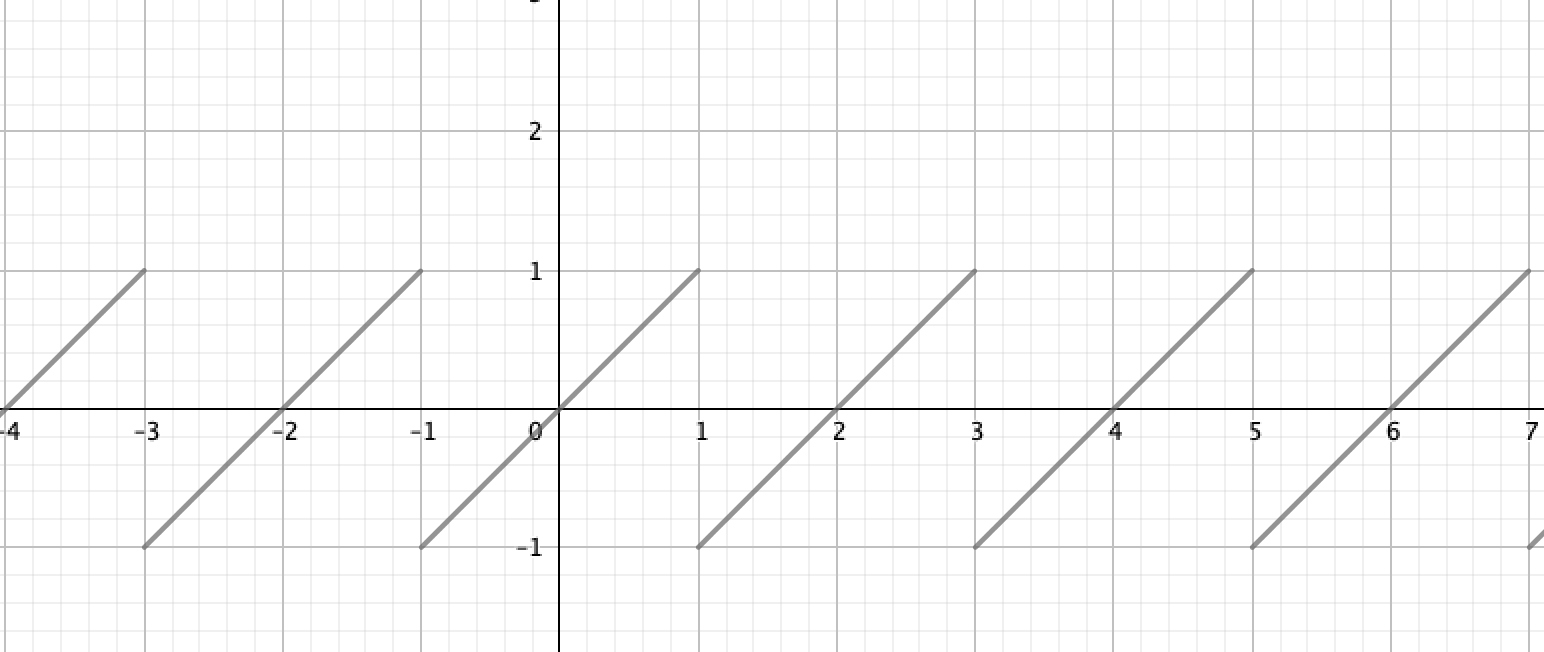
\includegraphics[width=0.5\linewidth]{./figures/e1_2.png}
  \caption{}
  \label{fig:e1_2}
\end{figure}

$f$ has been sketched on \textbf{\autoref{fig:e1_2}}. The Fourier series of this can, as it is a ``nice'' function be found by the formula:
\[ 
f(x) = a_0 + \sum_{n=1}^{\infty} \left( a_n \cos \frac{n \pi x}{L} + b_n \sin \frac{n \pi x}{L} \right)
.\]
Where $L = \frac{p}{2} = 1$ with $p = 2$ being the period of the function. The Fourier coefficients can be found by the Euler formulas:
\begin{align*}
  a_0 &= \frac{1}{2L} \int_{-L}^{L} f(x) \, \mathrm{d}x \\
  a_n &= \frac{1}{L}\int _{-L}^{L} f(x) \cos \frac{n \pi x}{L} \, \mathrm{d}x, \quad n = 1, 2, 3, \ldots  \\
  b_n &= \frac{1}{L} \int_{-L}^{L} f(x) \sin \frac{n \pi x}{L} \, \mathrm{d}x, \quad n = 1, 2, 3, \ldots
.\end{align*}
We start by solving for $a_0$ as:
\[ 
  a_0 =  \int_{-1}^{1} x \, \mathrm{d}x =  \left[ \frac{1}{2} x^2 \right]_{-1}^{1} = \cdot 0 = 0
.\]
We now solve for $a_n$ using integration by parts as:
\begin{align*}
  a_n &= \int_{-1}^{1} x \cos n\pi x \, \mathrm{d}x \\
  &= \left[ x \frac{\sin n\pi x}{n \pi} \right]_{-1}^{1} - \int_{-1}^{1} \frac{\sin n \pi x}{n \pi} \, \mathrm{d}x  \\
  &= \left( - \frac{1}{n\pi} \right) \int_{-1}^{1} \sin n \pi x \, \mathrm{d}x  \\
  &= \left[ - \frac{1}{n \pi} \right] \left[ - \frac{\cos n \pi x}{n \pi} \right]_{-1}^{1} \\
  &= 0
.\end{align*}
We similarly solve for $b_n$ as:
\begin{align*}
  b_n &= \int_{-1}^{1} x \sin n \pi x \, \mathrm{d}x  \\
      &= \left[ x \frac{- \cos n \pi x}{n \pi} \right]_{-1}^{1} - \int_{-1}^{1} \frac{- \cos n \pi x}{n \pi} \, \mathrm{d}x  \\
      &= \left( - \frac{2}{n\pi} \right) \cos n \pi + \frac{1}{n\pi} \left[ \frac{\sin n \pi x}{n \pi} \right]_{-1}^{1}\\
      &= \left( - \frac{2}{n \pi} \right) \cos n \pi
.\end{align*}
The full Fourier series therefore becomes:
\[ 
f(x) = \sum_{n = 1}^{\infty} \left( - \frac{2}{n \pi} \right) \cos n \pi \cdot \sin n \pi x
.\]


\exercise{3.}
Let $a \neq 0$ and $b \neq 0$. Let $f(x) = f(x + p_0)$ be a periodic function with period $p_0$. Is $f(ax + b)$ periodic? If yes, find a period. Give arguments for your answer.
\bigbreak
The $b$ only serves to translate the function $f(x)$ along the $x$-axis, this does not change the period. The value of $a$ corresponds to how ``quickly'' some value is reached, e.g. if $ax$ is an argument to a function a doubling of the value of $a$ will mean that the function will reach its maximum for a value of $x$ only half as big. I.e. there is an inverse relation between the size of $a$ and the period as:
\[ 
p_2 = \frac{p_1}{a}
.\]



\exercise{4.}
Calculate the left hand limit and the right hand limit of
\[ 
f(x) = \frac{\left| x \right|}{x}
\]
at $x = 0$.
\bigbreak
We start with the right-hand limit as:
\[ 
f(0+) = \lim_{h \to 0} \left( 0 + h \right) = \lim_{h \to 0} \frac{|h|}{h} = \lim_{h \to 0} \frac{h}{h} = 1
.\]
And now we can similarly do the left-hand limit as:
\[ 
f(0-) = \lim_{h \to 0} \left(  0- h \right) = \lim_{h \to 0} \frac{\left| -h \right|}{-h} = \lim_{h \to 0} \frac{h}{-h} = -1
.\]


\exercise{5.}
Calculate the left-hand derivative and the right-hand derivative of
\[ 
f(x) = x \left| x \right|
\]
at $x = 0$.
\bigbreak
We start with the right-hand derivative as:
\[ 
f'(0+) = \lim_{h \to 0} \frac{f(0 + h) - f(0)}{h} = \lim_{h \to 0} \frac{h |h|}{h} = \lim_{h \to 0} h = 0
.\]
And the left-hand derivative can likewise be computed as:
\[ 
f'(0-) = \lim_{h \to 0} \frac{f(0) - f(0 - h)}{h} = \lim_{h \to 0} \frac{-(-h) |-h|}{h} = \lim_{h \to 0} h = 0 
.\]

